\chapter{Client}

\section{Choix du framework}

\paragraph{}
Pour réaliser l’interface Web de notre application, nous avons opté pour la technologie \href{https://angular.io/}{\texttt{Angular}}.

\paragraph{}
Celui-ci nous servira à gérer l’aspect dynamique de l’application web réalisée en \texttt{HTML} et \texttt{CSS}, comme la navigation d’une page de l’interface à une autre ou le passage de paramètres entre pages. \texttt{Angular} est un framework web développé en \texttt{TypeScript} et est l’un des plus utilisés pour le développement \textit{front-end} des applications web. Les principaux avantages d’\texttt{Angular} sont qu’il est mis à jour très régulièrement par les développeurs de Google, qu’il dispose d’une très bonne documentation et que le développement en \texttt{TypeScript} est stable, rapide et facile.

\paragraph{}
\texttt{Angular}, \texttt{HTML} et \texttt{CSS} sont des technologies largement utilisées par les développeurs et relativement simples d’utilisation. En outre, nous avons déjà été amenés à les utiliser dans des projets précédents, nous partons donc avec des bases. Nous avons fait le choix de la simplicité et de l’utilisation de technologies que nous avons déjà abordées afin de faciliter et d’accélérer la réalisation de l’interface, pour être en mesure de proposer un prototype fonctionnel pour la première itération le 27 février.

%-------------------------------------------------------------------------------
\section{Les différents composants de l'interface}

\paragraph{Première itération}
Pour la première itération, l’interface est réduite à sa forme la plus simple qui répond au cahier des charges, à savoir ouvrir un document de travail et valider ou invalider les transcriptions. L’IHM aura donc deux composants : la page d’accueil et la page de validation des annotations.

\paragraph{}
La page d’accueil permet à l’utilisateur de choisir le projet sur lequel il veut travailler ainsi que d'en créer de nouveaux en choisissant les documents qui le composent. Un projet possède plusieurs documents qui possèdent eux-mêmes plusieurs pages contenant les imagettes (\textit{PEA\_GEN\_6}). Cette page possède une liste des projets qui ont été ouverts auparavant dans l’application, ainsi qu’un bouton pour en créer un nouveau. Un clic sur ce bouton ouvre une nouvelle fenêtre pour que l’utilisateur parcoure ses documents et fasse son choix (spécifications \textit{PEA\_GEN\_7} et \textit{PEA\_GEN\_8}).

\newpage{}
\begin{mdframed}[frametitle={Figure 1 : Maquette de la page d'accueil de l'IHM}, innerbottommargin=10]
\begin{center}
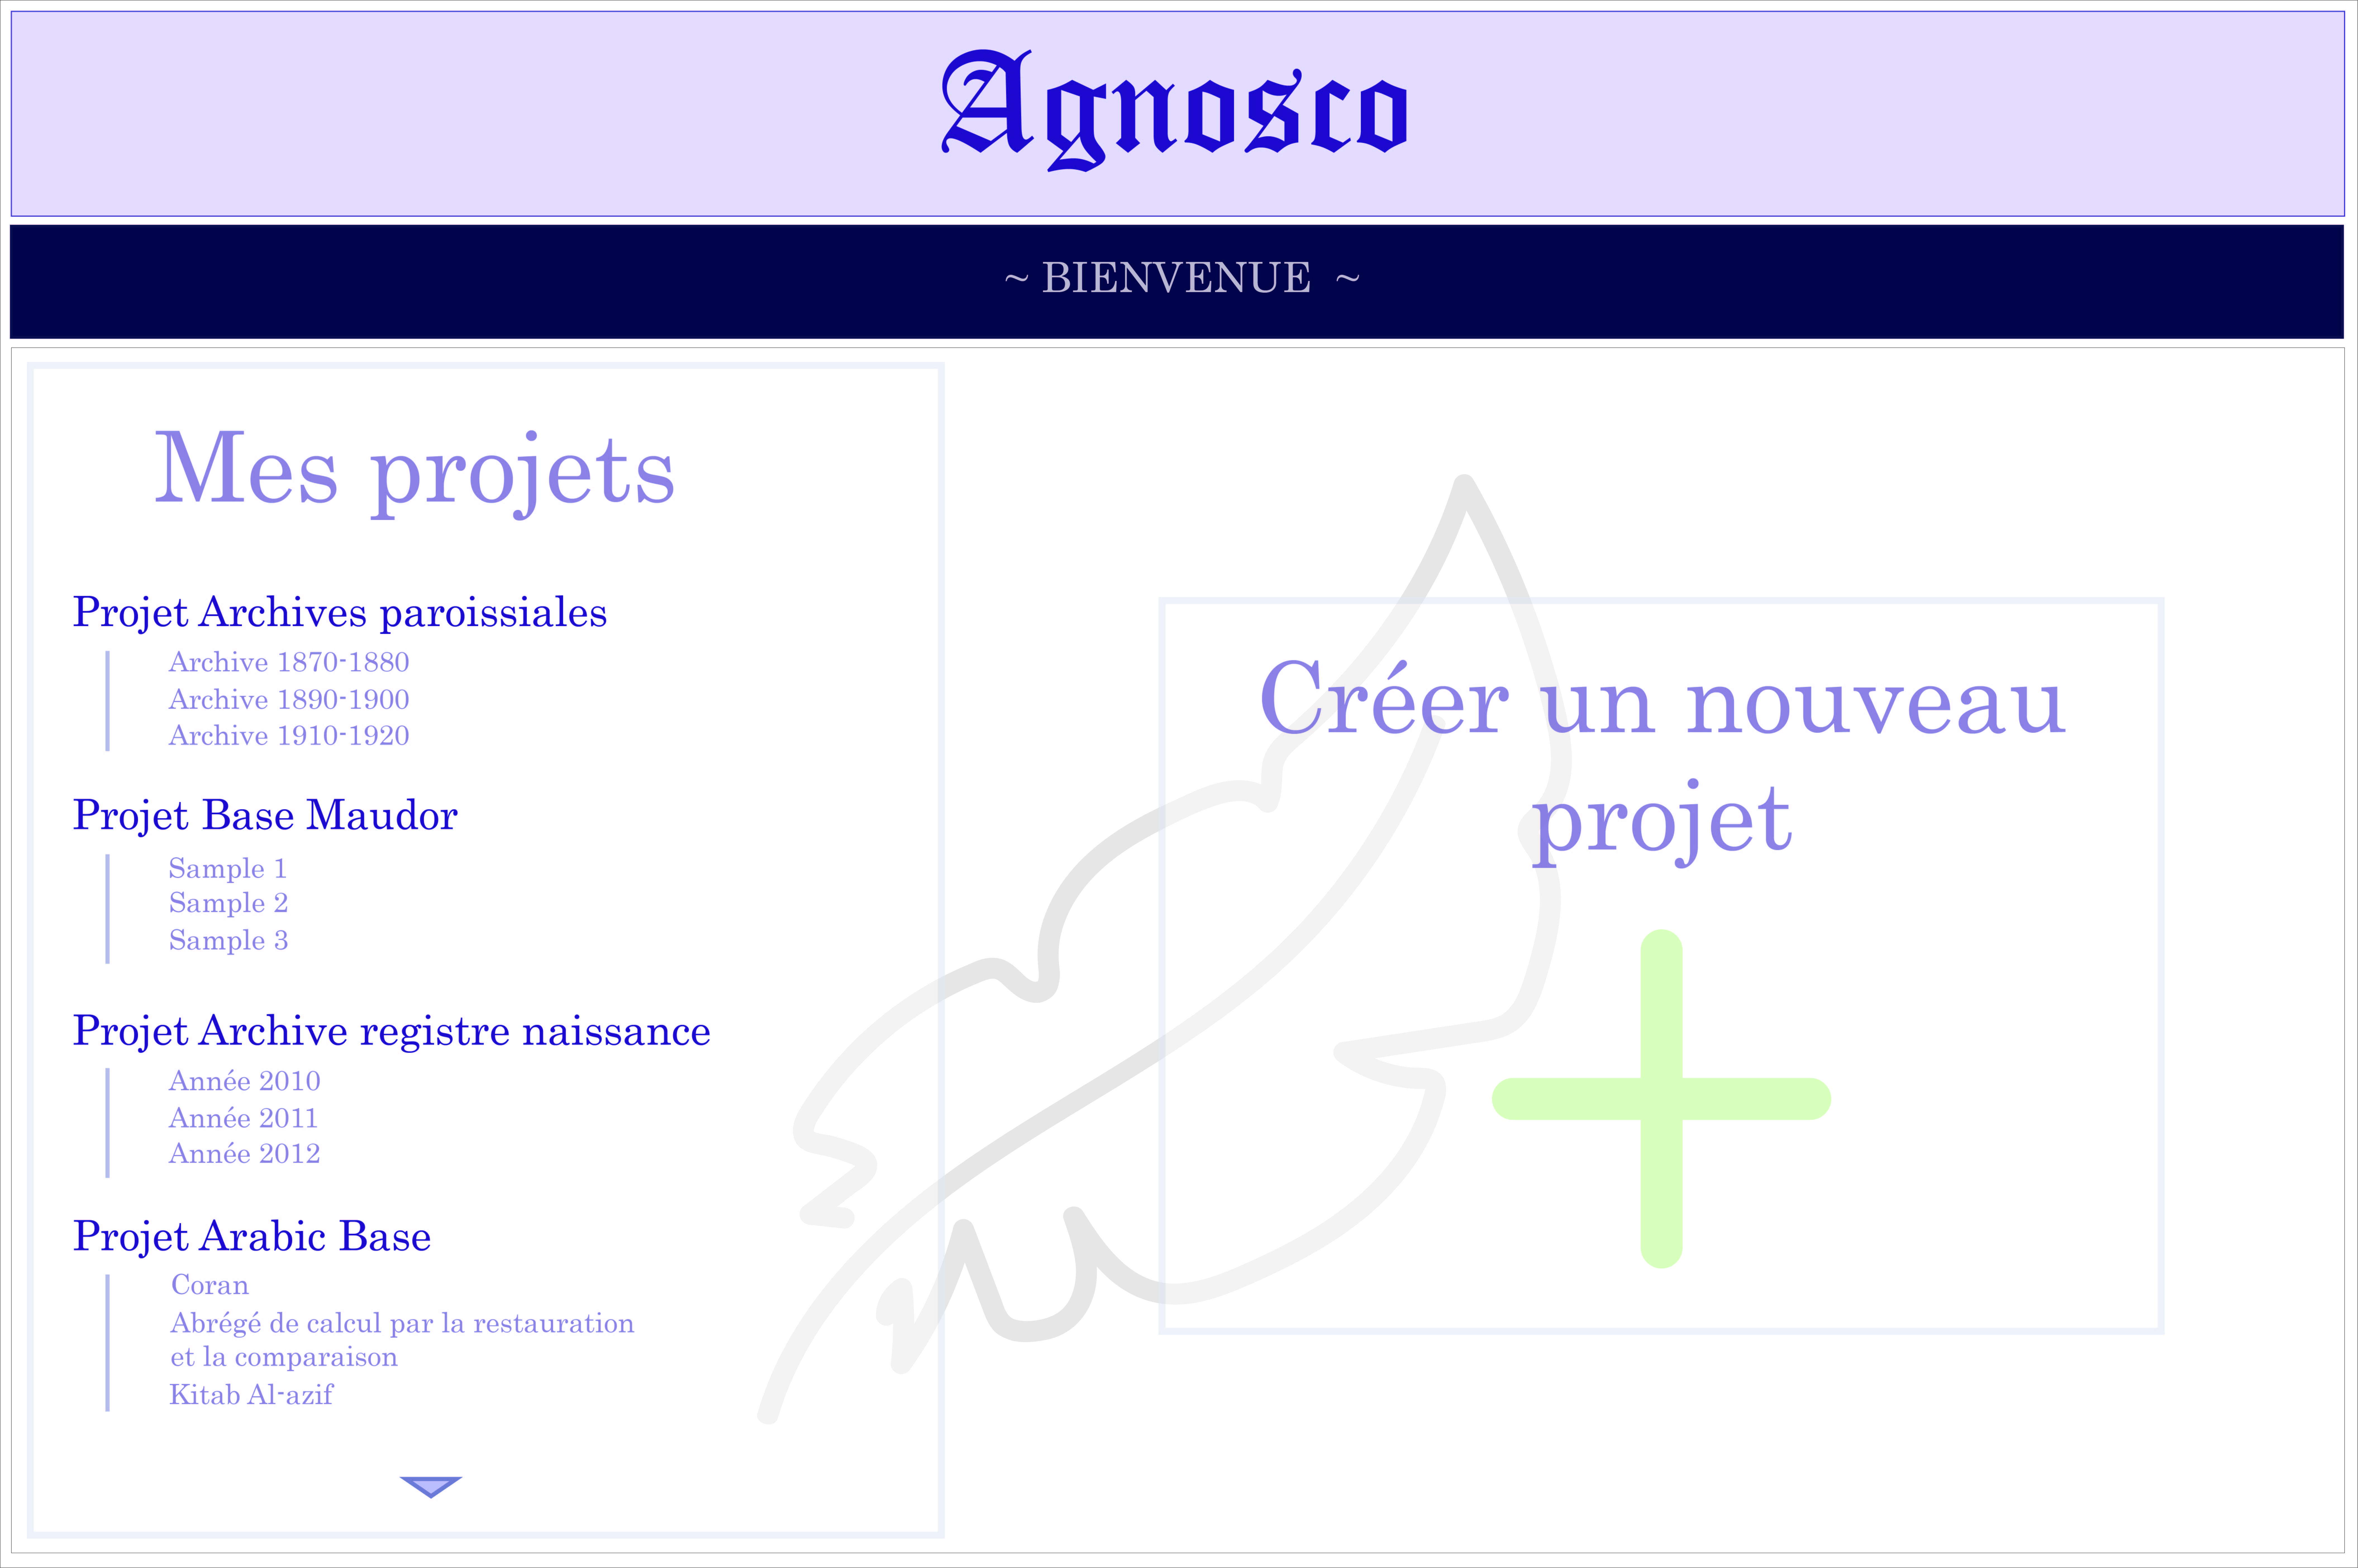
\includegraphics[scale=0.04]{assets/maquetteIHMaccueil.jpg}
\end{center}
\end{mdframed}

\paragraph{}
La page de validation (spécifications \textit{PVAL\_1} à \textit{PVAL\_7}), comme son nom l’indique, permet de valider ou d’invalider les transcriptions de la base de données relatives au document ouvert (\textit{PEA\_GEN\_1}). Ces transcriptions ayant été réalisées par des humains, elles sont considérées comme vraies et l’utilisateur pourrait les invalider seulement s’il manque des mots ou si l’imagette est jugée peu pertinente pour l’apprentissage (par exemple, si le texte est presque illisible ou si l’imagette ne contient pas de texte du tout).
\newline{}
Pour ce faire, les imagettes sont affichées les unes à la suite des autres et chacune possède sa transcription située dans une zone de texte en dessous. Les imagettes sont affichées par groupe de cinq ou six. Une croix à côté de chaque imagette permet à l’utilisateur d’invalider le couple imagette-transcription correspondant. Un simple appui sur la touche \texttt{Entrée} valide l’ensemble des couples affichés sur la page, afin de permettre à l’utilisateur de réaliser la validation le plus rapidement possible. Des flèches gauche et droite permettent de se déplacer dans les groupes d’imagettes pour parcourir l’ensemble des pages du document. Enfin, une icône en haut à gauche renvoie à la page d’accueil.

\begin{mdframed}[frametitle={Figure 2 : Maquette de la page de validation des annotations}, innerbottommargin=10]
\begin{center}
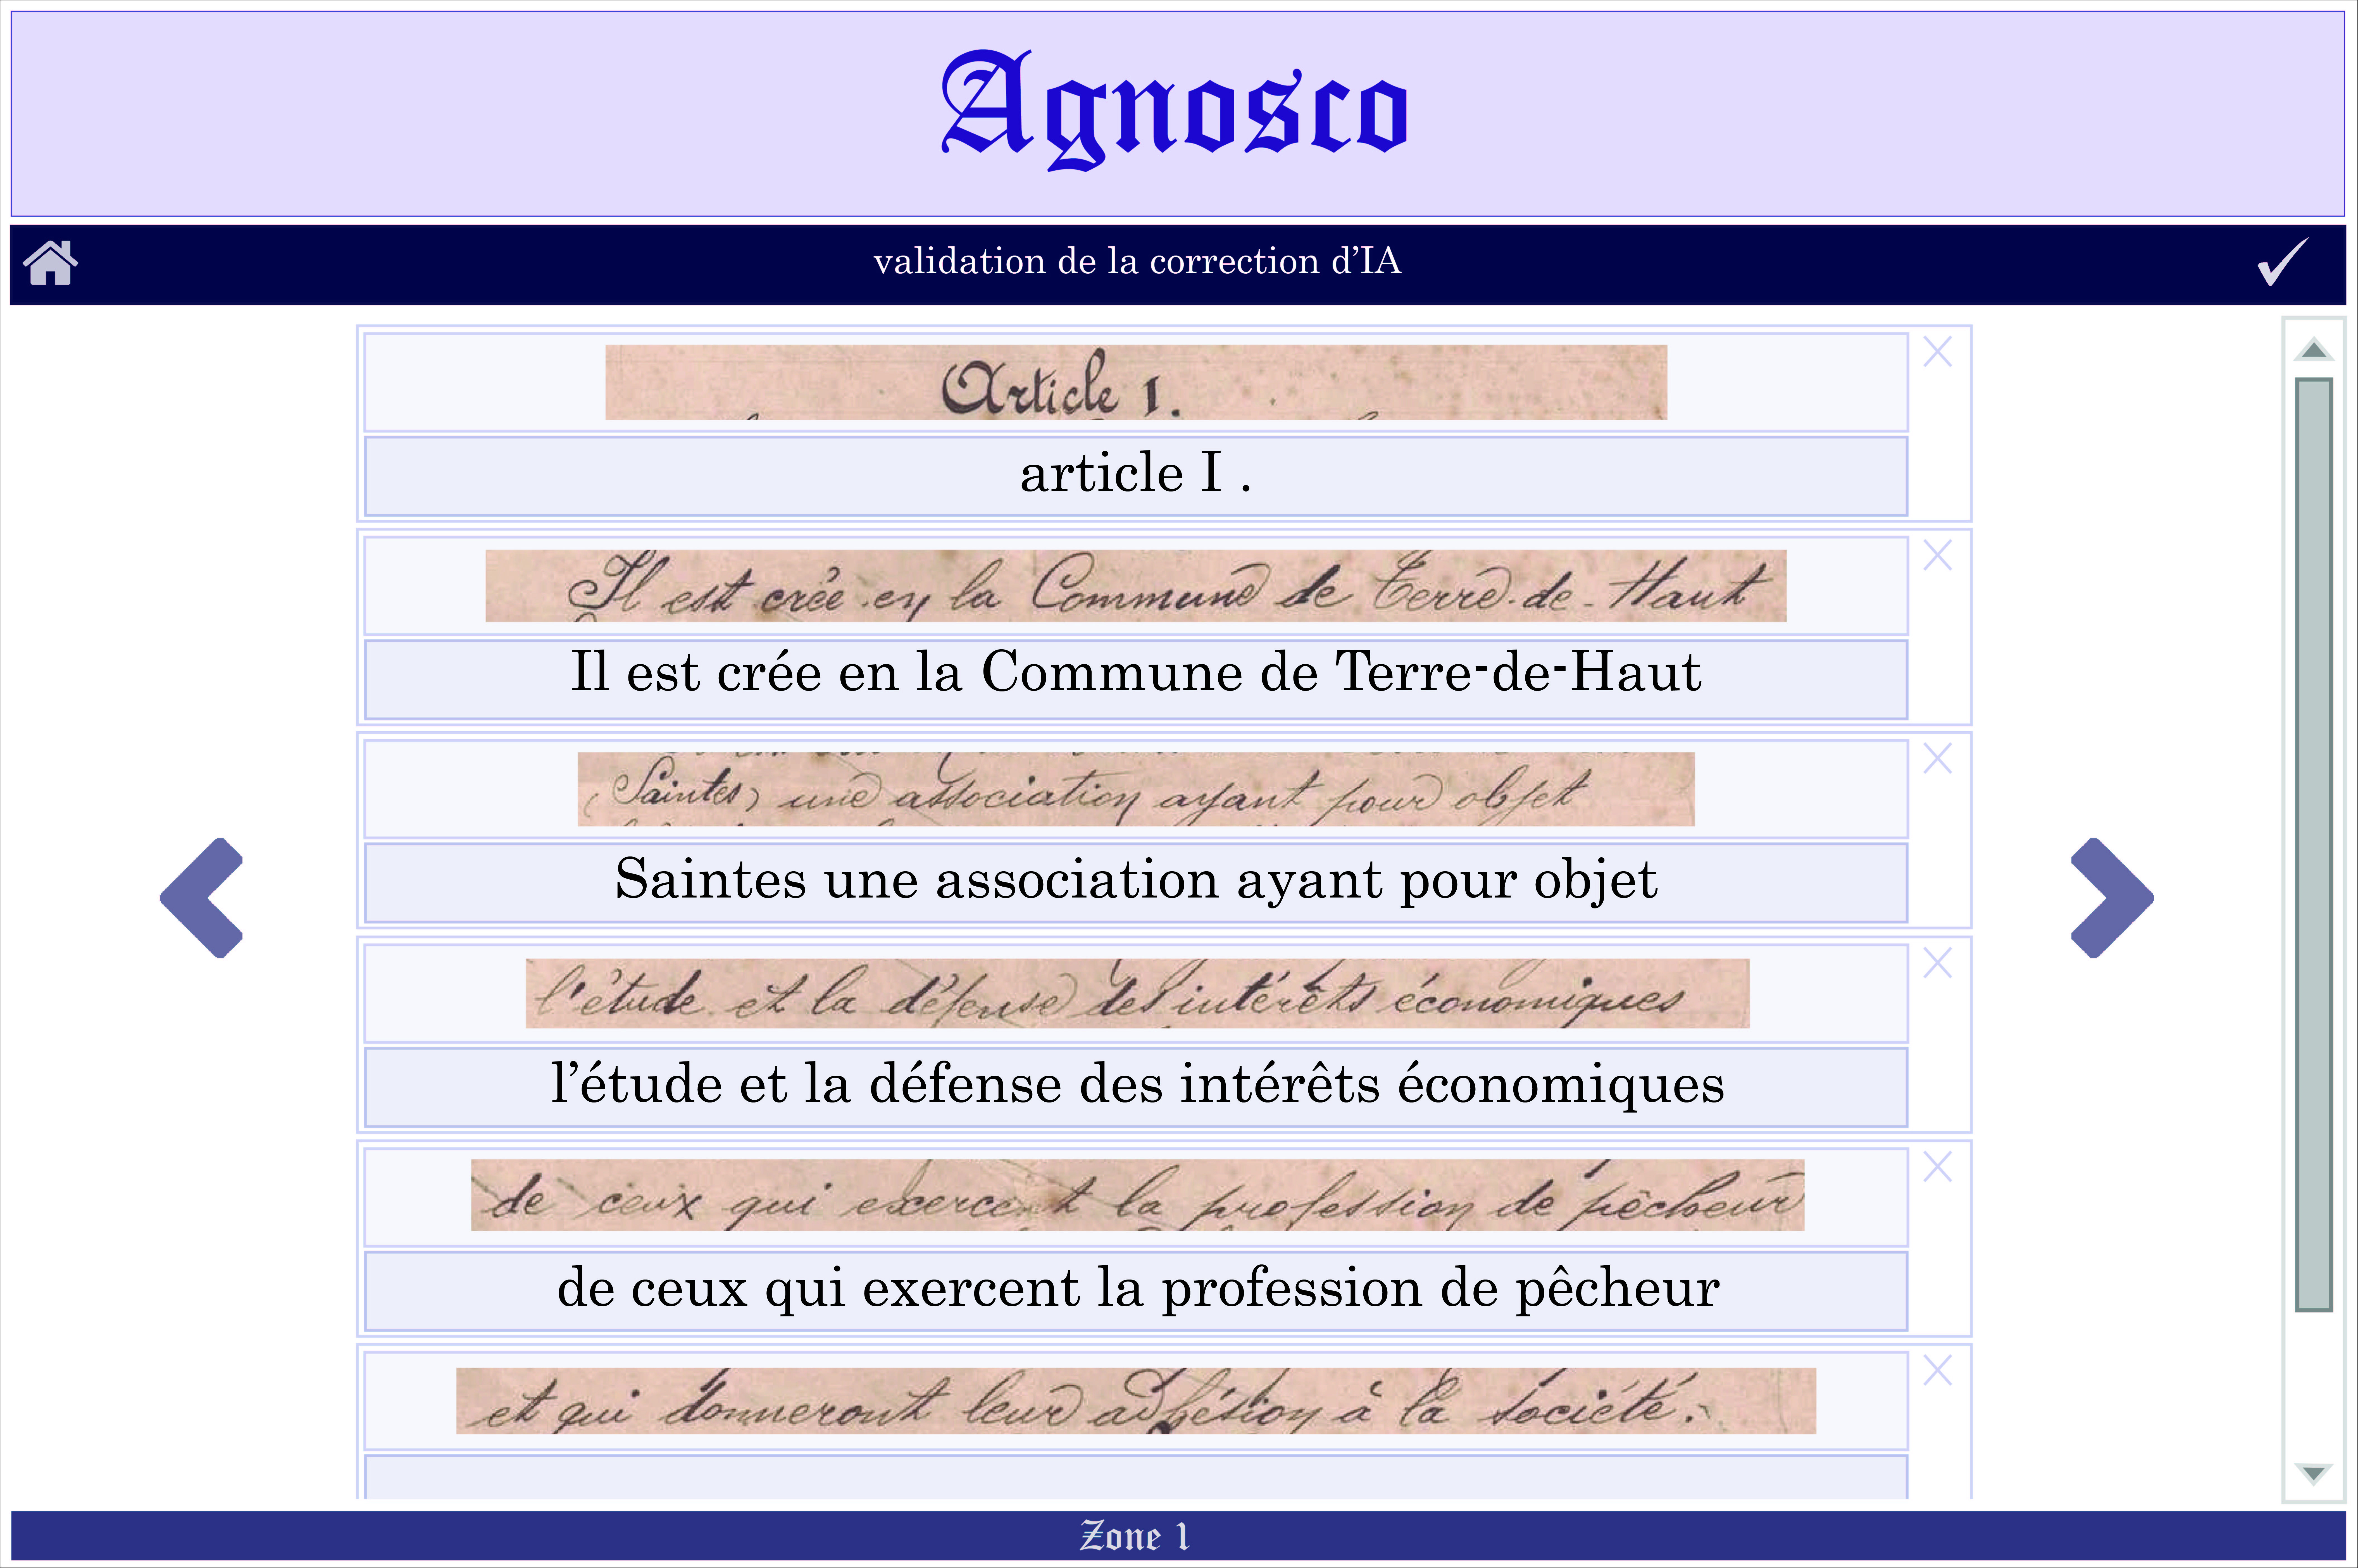
\includegraphics[scale=0.04]{assets/maquetteIHMvalidation1.jpg}
\end{center}
\end{mdframed}

\newpage{}

\paragraph{Deuxième itération}
Pour la deuxième itération, nous implémenterons les fonctionnalités supplémentaires décrites dans les rapports précédents.

\paragraph{}
Nous proposerons tout d’abord une page de découpe des zones ou des paragraphes du document à l’aide d’outils graphiques regroupés dans une zone à droite de la page (spécifications \textit{PDEC\_OD\_1} à \textit{PDEC\_OD\_11}). Il y aura un outil pour créer un nouvelle sélection sous la forme d’un quadrilatère, un outil pour déplacer une sélection existante, un autre pour zoomer et dézoomer, un pour annuler ou refaire la dernière action, un outil pour réinitialiser la découpe et supprimer toutes les sélections réalisées et enfin, un dernier outil “premier jet” permettant de lancer un reconnaisseur de lignes sur les zones découpées. Ce dernier permet de vérifier que les découpes ont bien été réalisées, soit que les lignes sont bien reconnues dans leur intégralité et qu'aucune partie du texte scanné n’est manquante.
\newline{}
La bannière en haut de la page contiendra plusieurs boutons de navigation. Un premier bouton permettra de revenir à l’accueil, comme dans toutes les pages de l’interface. Un autre exportera la page découpée vers un reconnaisseur d’écriture manuscrite en envoyant les couples imagettes - transcriptions au reconnaisseur (\textit{PDEC\_OD\_12}). Tout à droite, un autre bouton permettra à l’utilisateur de passer à la page de transcription manuscrite (\textit{PDEC\_OD\_12}).

\begin{mdframed}[frametitle={Figure 3 : Maquette de la page de découpe des zones}, innerbottommargin=10]
\begin{center}
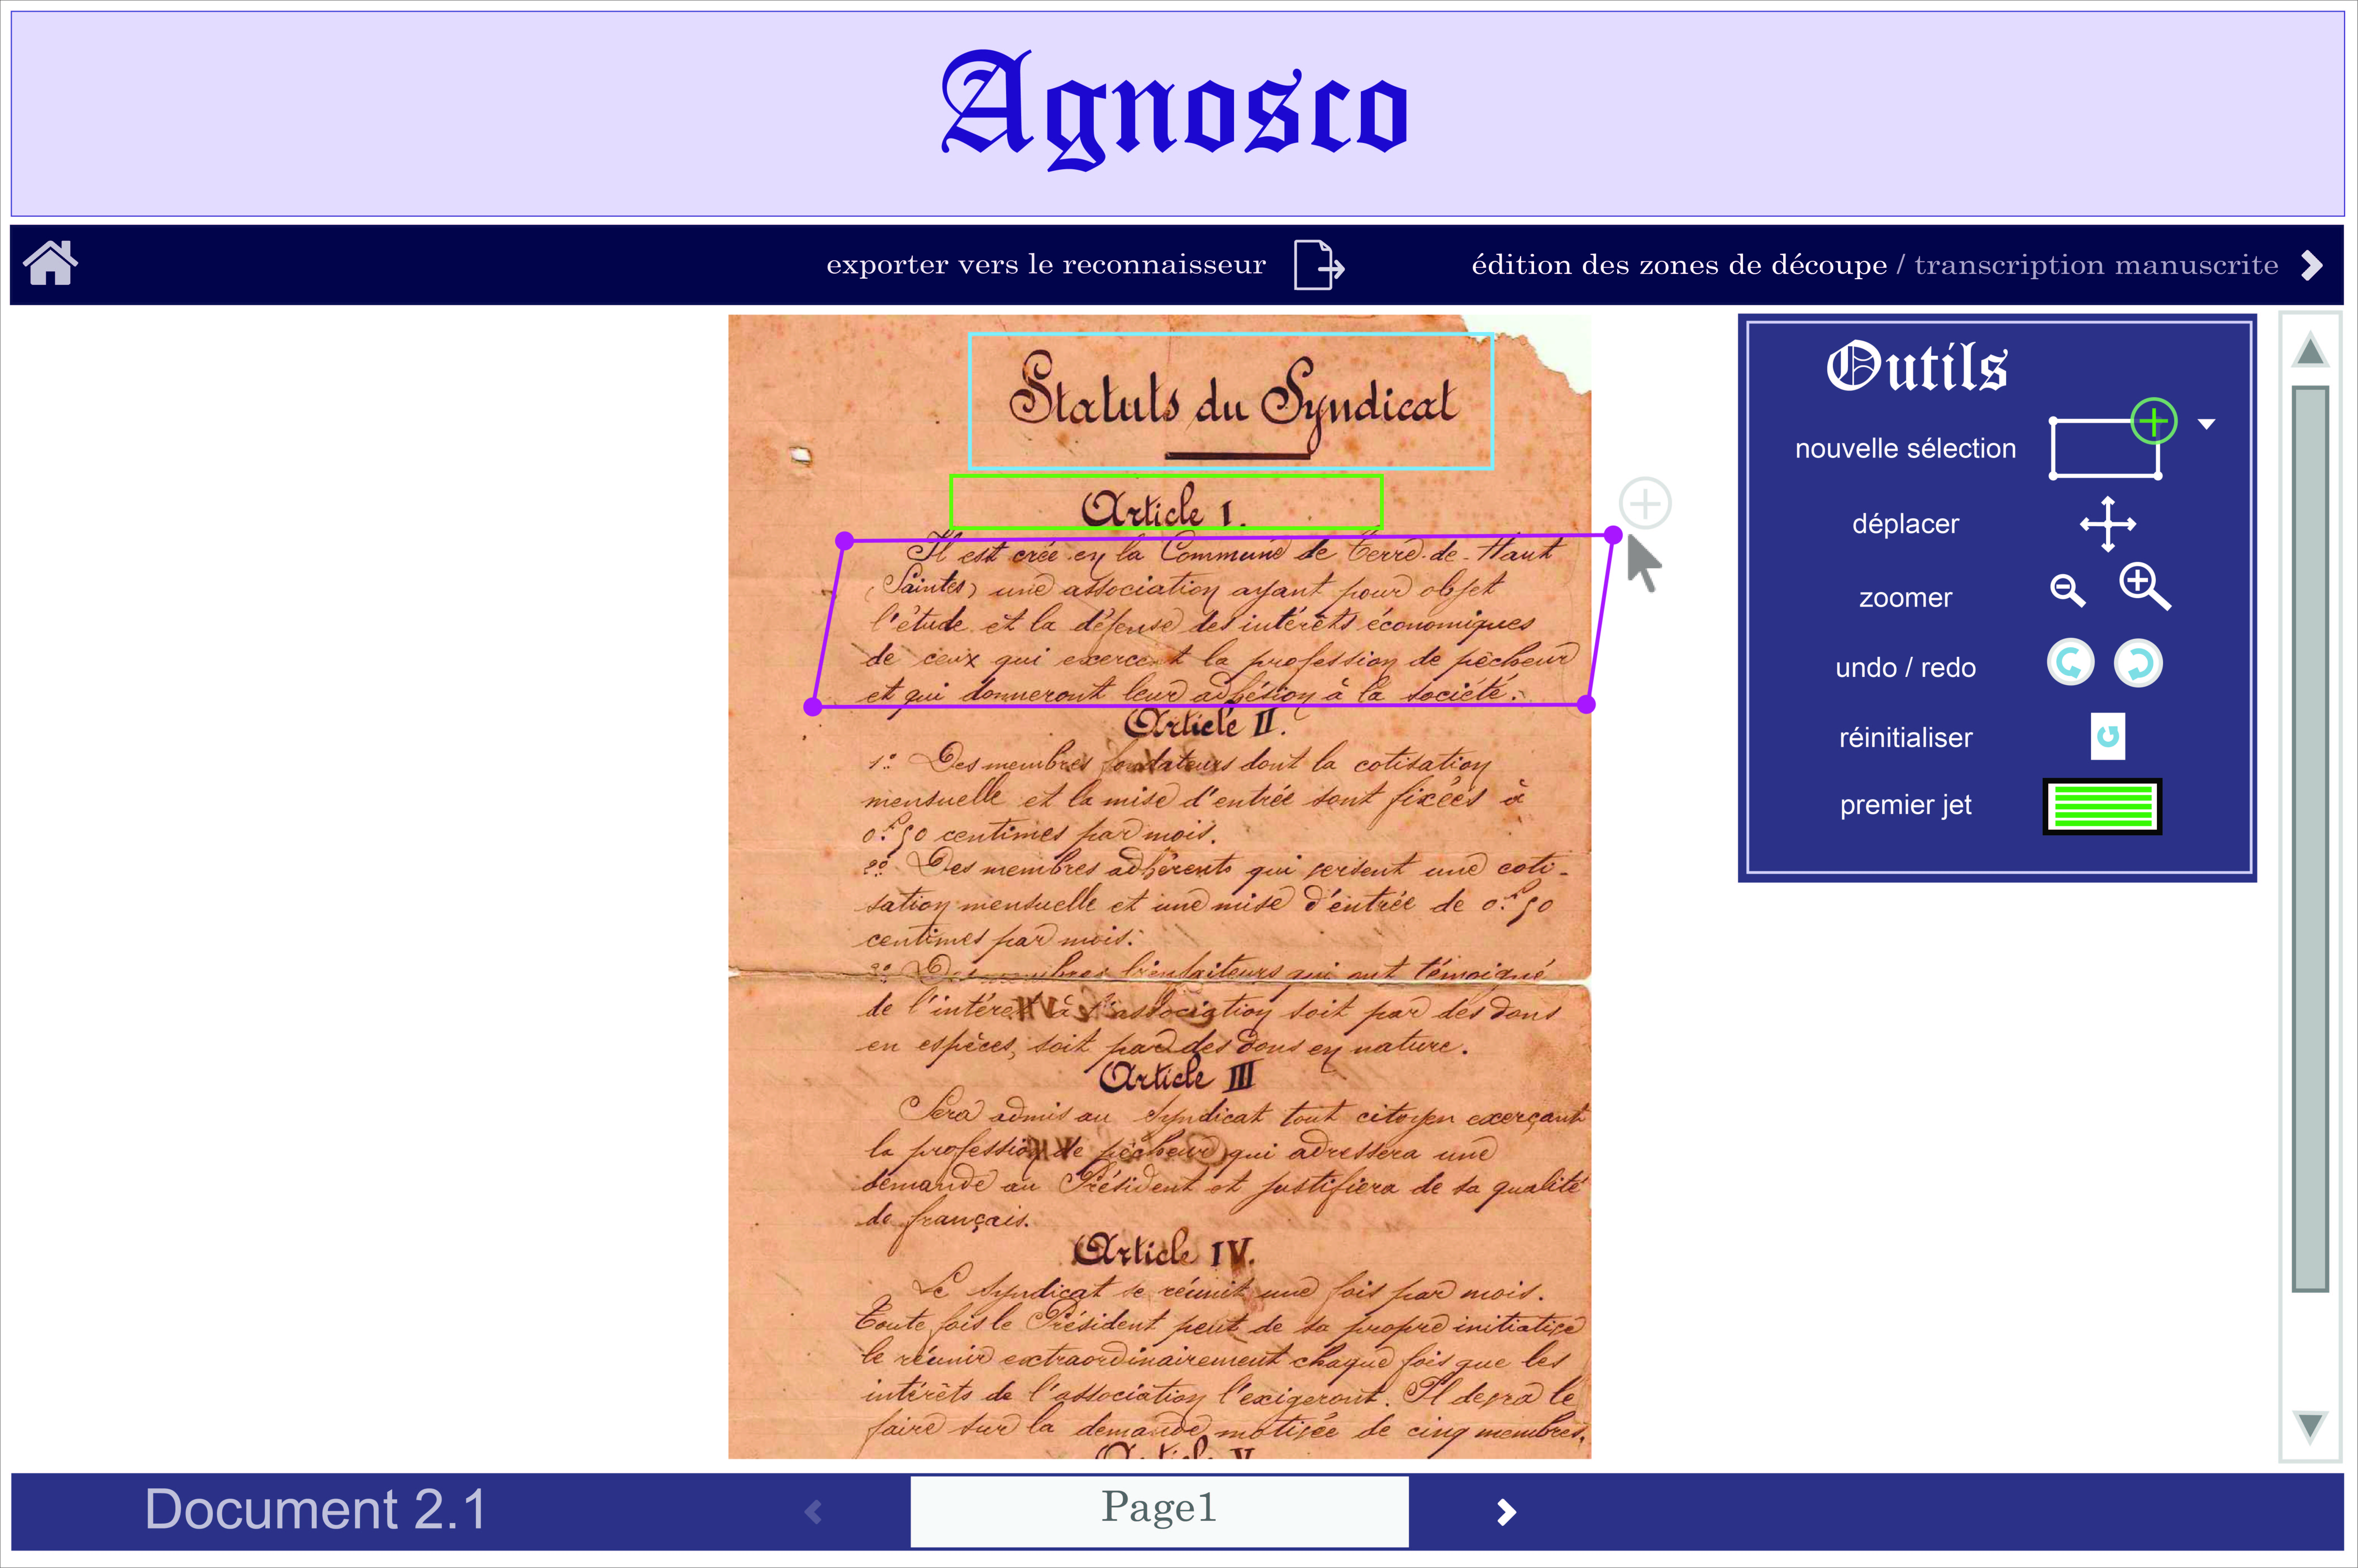
\includegraphics[scale=0.04]{assets/maquetteIHMdecoupes.jpg}
\end{center}
\end{mdframed}

\paragraph{}
Lors de l’ouverture d’un nouveau document de travail, il devra être possible d’utiliser des manuscrits scannés qui ne possèdent pas de vérités-terrain. L’utilisateur aura alors la possibilité d’annoter le manuscrit manuellement ou de le faire passer par un reconnaisseur d’écriture après avoir découpé les zones du manuscrit via la page de découpe de l’interface.

\paragraph{}
L’interface possèdera donc une page d’annotation manuelle (\textit{PEA\_GEN\_2}). Les imagettes d’une même zone seront affichées à la suite dans la fenêtre centrale, avec une zone de texte pour la transcription située sous chaque imagette. Le curseur sera positionné automatiquement sur la première transcription affichée (\textit{PEMA\_1}), l’utilisateur devra taper la transcription manuellement au clavier puis appuyer sur la touche \texttt{Entrée} pour passer à la transcription suivante (\textit{PEMA\_2}). Lorsque toutes les imagettes d’une zone ont été annotées, on passe automatiquement aux imagettes de la zone suivante à l’appui sur \texttt{Entrée} de la dernière transcription. Le but est de minimiser les actions requises par l’utilisateur, pour qu’il n’utilise que son clavier. Il peut néanmoins positionner son curseur sur la transcription de son choix à l’aide de sa souris.
\newline{}
Une croix à droite de chaque imagette permet de supprimer le couple imagette-transcription de la base d’apprentissage si le couple est jugé peu pertinent (\textit{PEMA\_6}). Après l’appui sur ce bouton, le couple est flouté mais toujours visible et la croix est remplacée par une flèche montante qui permet de réintroduire le couple supprimé dans la base d’apprentissage.
\newline{}
Cette page de l’interface possèdera également une fenêtre à droite montrant la page courante en entier, avec toutes ses zones de découpe affichées en surbrillance. Un rectangle parcourera la page au fur et à mesure de la transcription pour indiquer la position courante dans la page.
\newline{}
Sous cette fenêtre de visualisation de la page, l’interface proposera une fenêtre de navigation dans les différents documents, permettant à l’utilisateur d’ouvrir un autre document de travail à tout moment.
\newline{}
Dans la bannière en haut de la page, un bouton permettra à l’utilisateur de revenir à la page de découpe des zones ou encore d’avancer à la page de validation finale des transcriptions, tandis qu’un autre renverra à l’accueil.

\begin{mdframed}[frametitle={Figure 4 : Maquette de la page d'annotation manuelle}, innerbottommargin=10]
\begin{center}
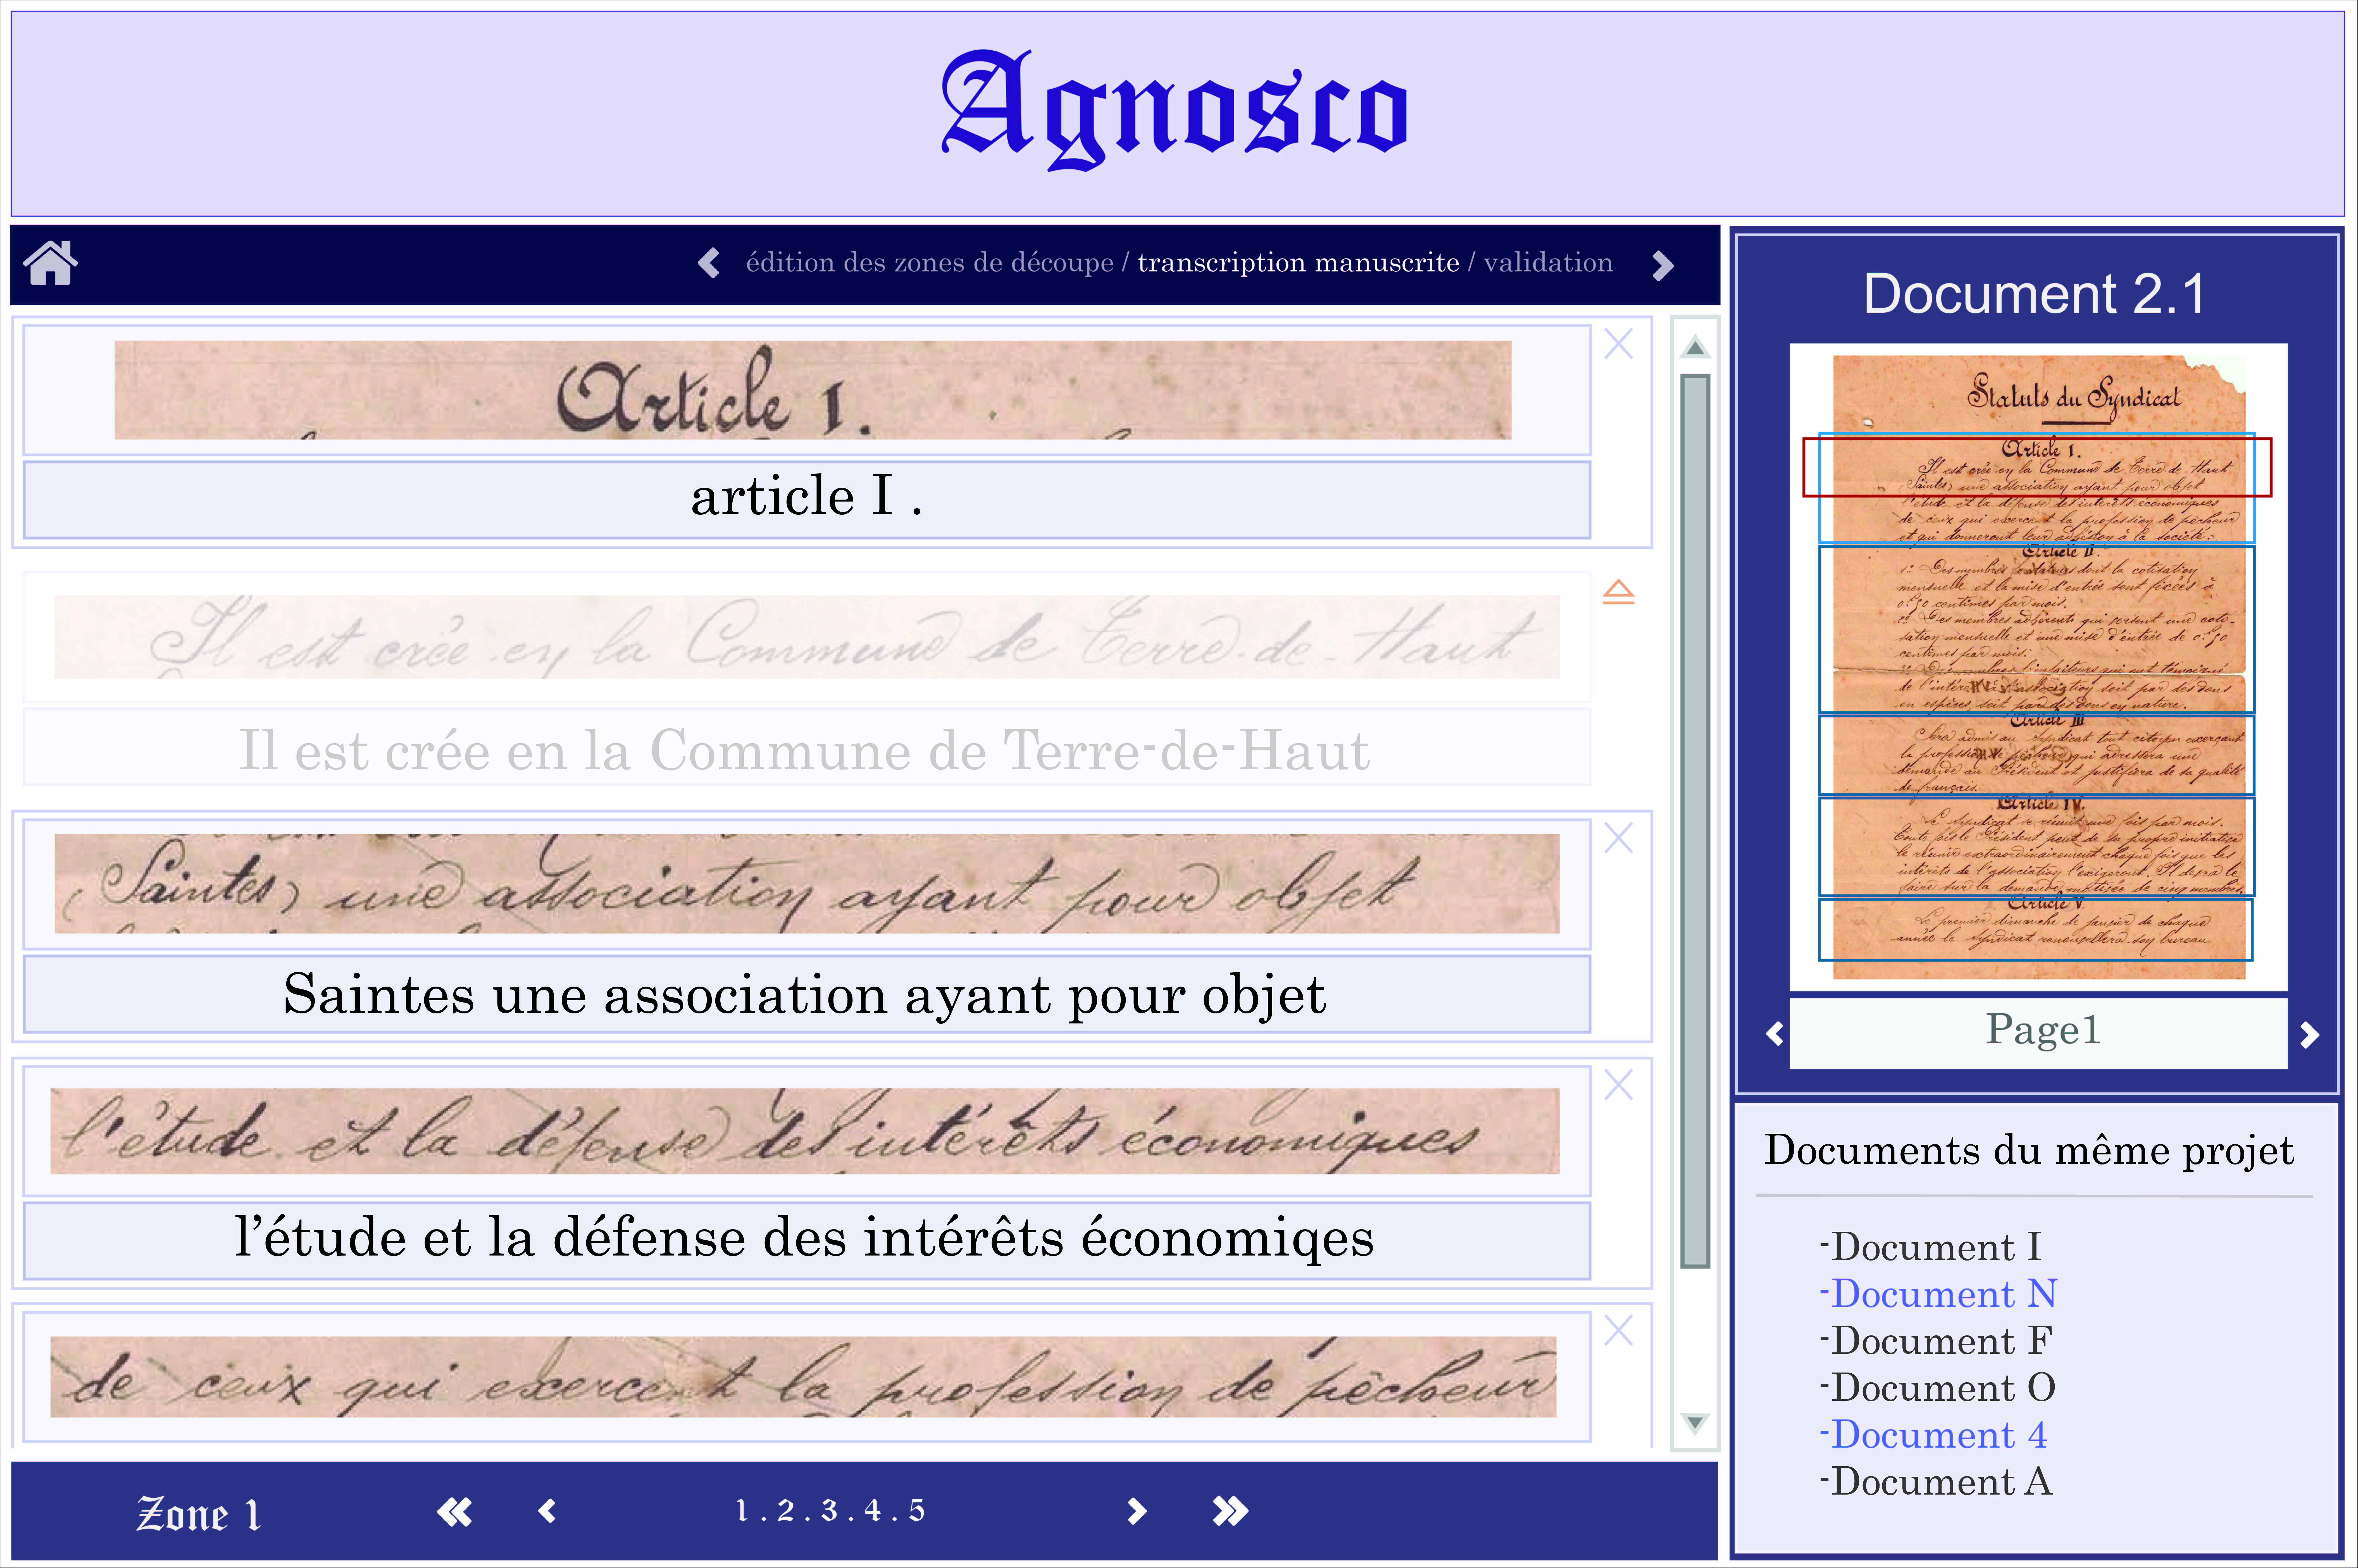
\includegraphics[scale=0.04]{assets/maquetteIHMtranscriptionmanu.jpg}
\end{center}
\end{mdframed}

\paragraph{}
Si l’utilisateur souhaite faire passer le manuscrit par le reconnaisseur plutôt que de l’annoter manuellement, il pourra visualiser et corriger les résultats de la reconnaissance via la page dédiée de l’interface (\textit{PEA\_GEN\_3}). Cette page sera sensiblement similaire à la page d’annotation manuelle, la différence principale résidant dans le fait que des transcriptions réalisées par le reconnaisseur seront déjà présentes sous chaque imagette. Le curseur se positionnera automatiquement sur la première transcription et un simple appui sur la touche \texttt{Entrée} passera à la transcription suivante. L’utilisateur pourra modifier manuellement la transcription courante en tapant ses modifications au clavier (spécifications \textit{PCORIA\_1} à \textit{PCORIA\_5}).
\newline{}
Dans la bannière du haut de la page, un bouton renverra à l’accueil et un autre permettra la navigation vers la page de validation finale des transcriptions.

\newpage{}

\begin{mdframed}[frametitle={Figure 5 : Maquette de la page de visualisation des transcriptions du reconnaisseur}, innerbottommargin=10]
\begin{center}
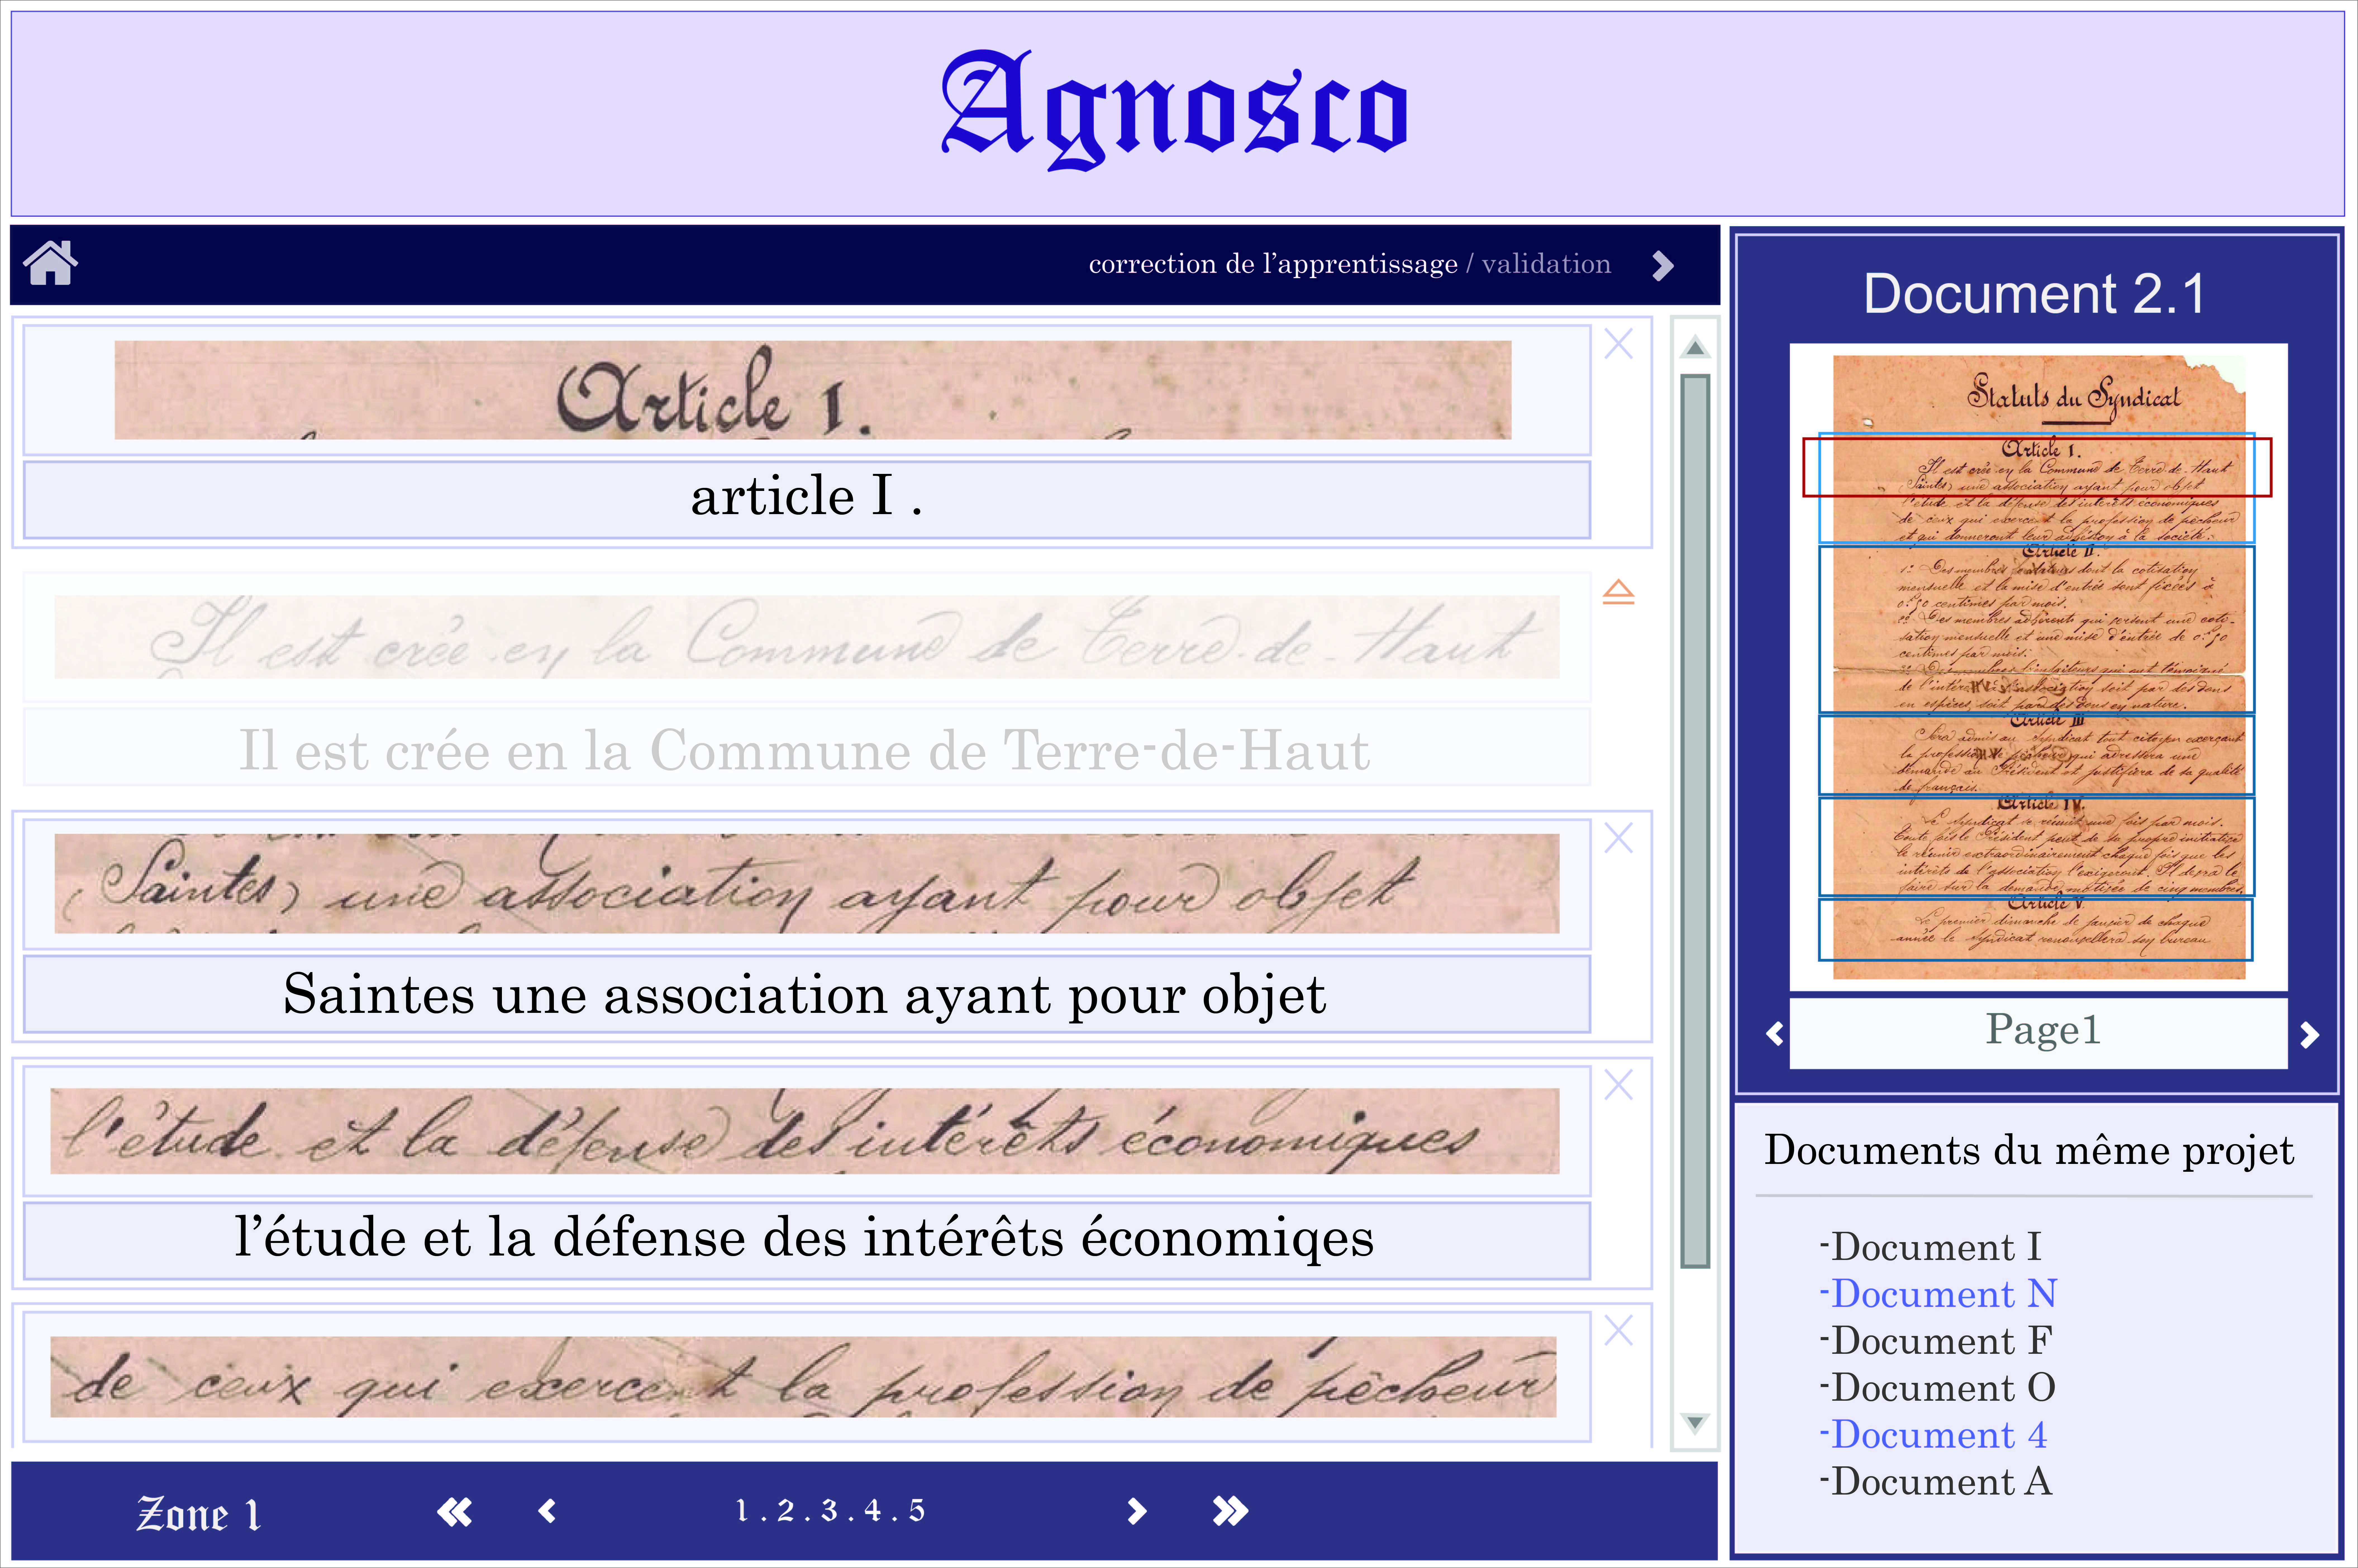
\includegraphics[scale=0.04]{assets/maquetteIHMcorrectionIA.jpg}
\end{center}
\end{mdframed}

\paragraph{}
Enfin, la dernière page de l’interface sera la page de validation qui a déjà été réalisée lors de la première itération. Deux modifications y seront apportées pour la deuxième itération.
\newline{}
Tout d'abord, une fenêtre sera ajoutée pour visualiser la page courante en miniature avec ses zones de découpe affichées par dessus ainsi qu’un rectangle montrant la position courante de l’utilisateur, afin que ce dernier ait constamment accès à sa position dans le document.
\newline{}
Ensuite, la bannière en haut de la page affichera si les transcriptions ont été réalisées manuellement par un humain ou par le reconnaisseur d'écriture, car l'attention fournie par l'utilisateur devrait être moindre pour un manuscrit annoté manuellement où les fautes sont théoriquement moins nombreuses. Savoir si la transcription a été faite manuellement ou par le reconnaisseur permettrait d'augmenter la rapidité de la validation finale.

\begin{mdframed}[frametitle={Figure 6 : Maquette de la page de validation finale lors de la deuxième itération}, innerbottommargin=10]
\begin{center}
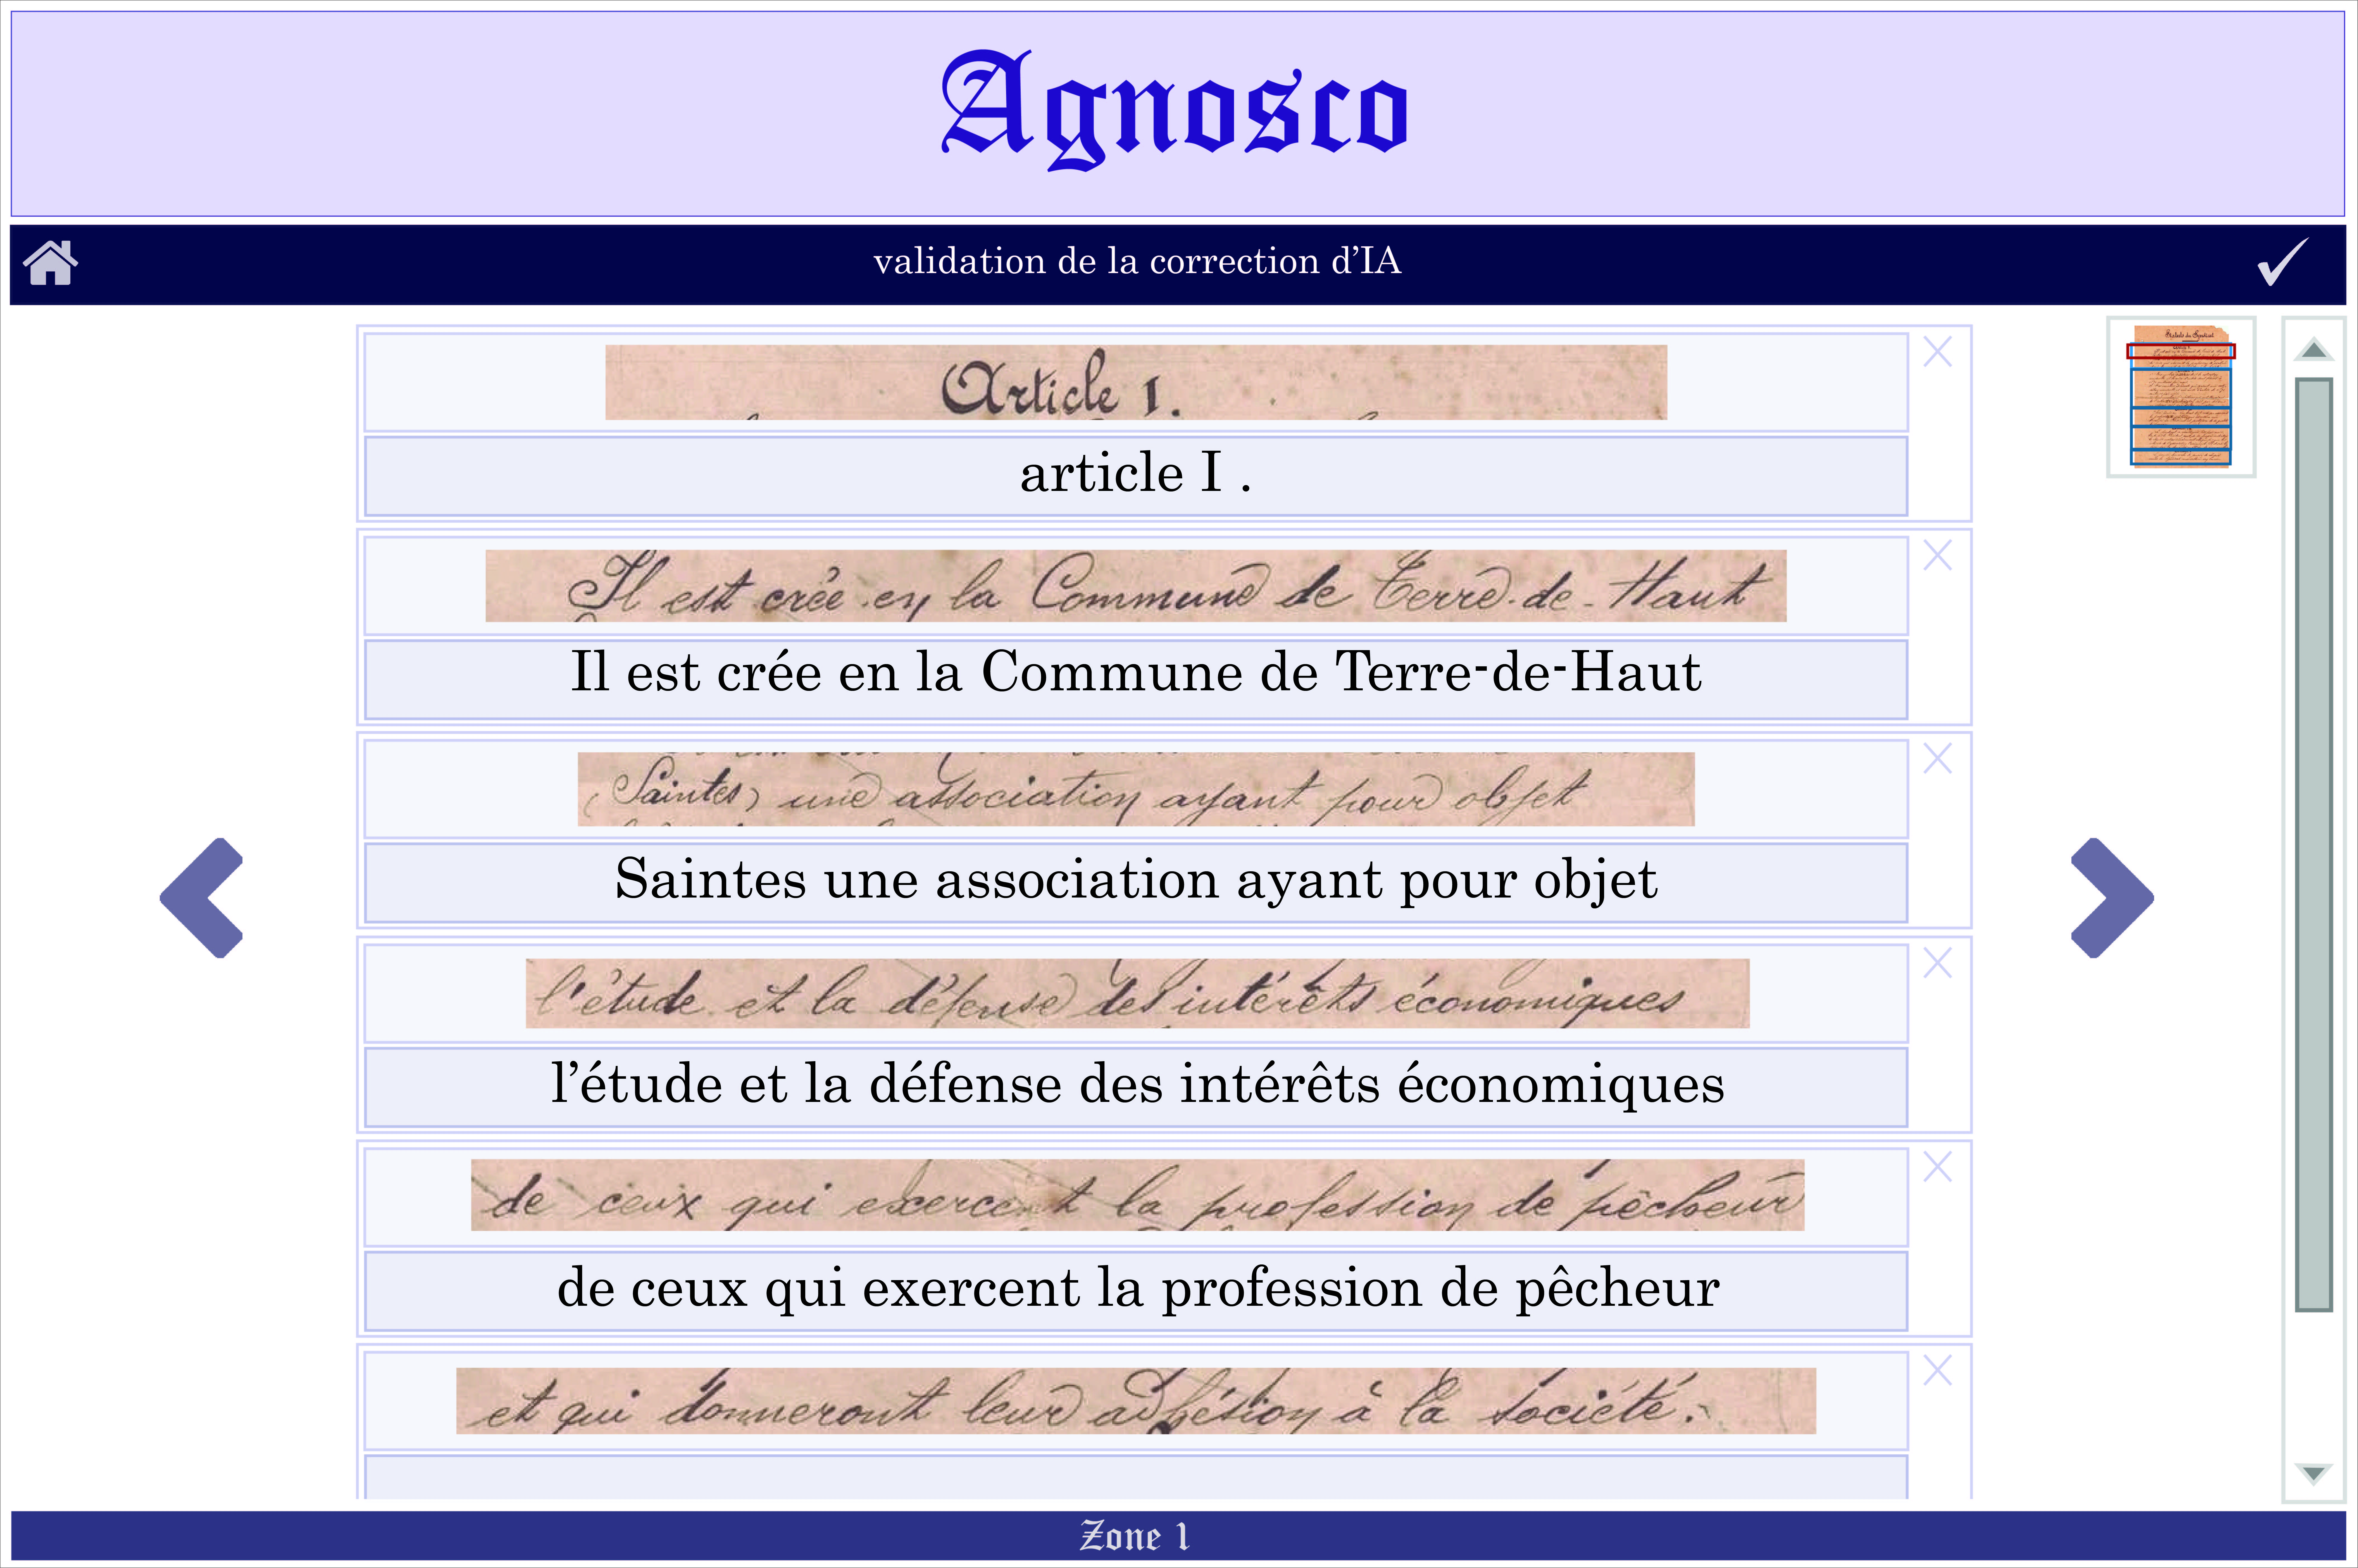
\includegraphics[scale=0.04]{assets/maquetteIHMvalidationIA.jpg}
\end{center}
\end{mdframed}

\paragraph{}
En résumé, à la fin de la deuxième itération, nous aurons cinq composants différents : la page d’accueil, la page de découpe des zones du document, la page d’annotation manuelle, la page de visualisation de la reconnaissance et la page de validation finale des transcriptions.


%-------------------------------------------------------------------------------
\section{Interactions}

\paragraph{Interactions entre les composants de l'interface}
L’utilisateur peut naviguer entre les différents composants via les boutons de l’interface.
\newline{}
Tout d’abord, une icône permettant de revenir à la page d’accueil sera présente en haut à gauche de chaque page - à l’exception de la page d’accueil. Sur cette dernière, le choix du document ouvre celui-ci dans la page de l’interface qui lui correspond, soit :

\begin{itemize}
\item la page de découpe si aucun travail n’a été réalisé au préalable sur ce document ;
\item la page d’annotation manuelle si les découpes ont déjà été réalisées et que l’utilisateur n’a pas exporté le document vers le reconnaisseur ;
\item la page de visualisation des transcriptions du reconnaisseur si une reconnaissance a été réalisée sur le document ;
\item ou la page de validation finale si toutes les transcriptions ont déjà été renseignées.
\end{itemize}

Des boutons de navigation dans les différentes pages sont également présents sur certaines pages, comme décrit dans la partie précédente. Les interactions sont visibles dans le schéma ci-dessous :

\begin{mdframed}[frametitle={Figure 7 : Schéma des interactions entre les différents composants de l'IHM}, innerbottommargin=10]
\begin{center}
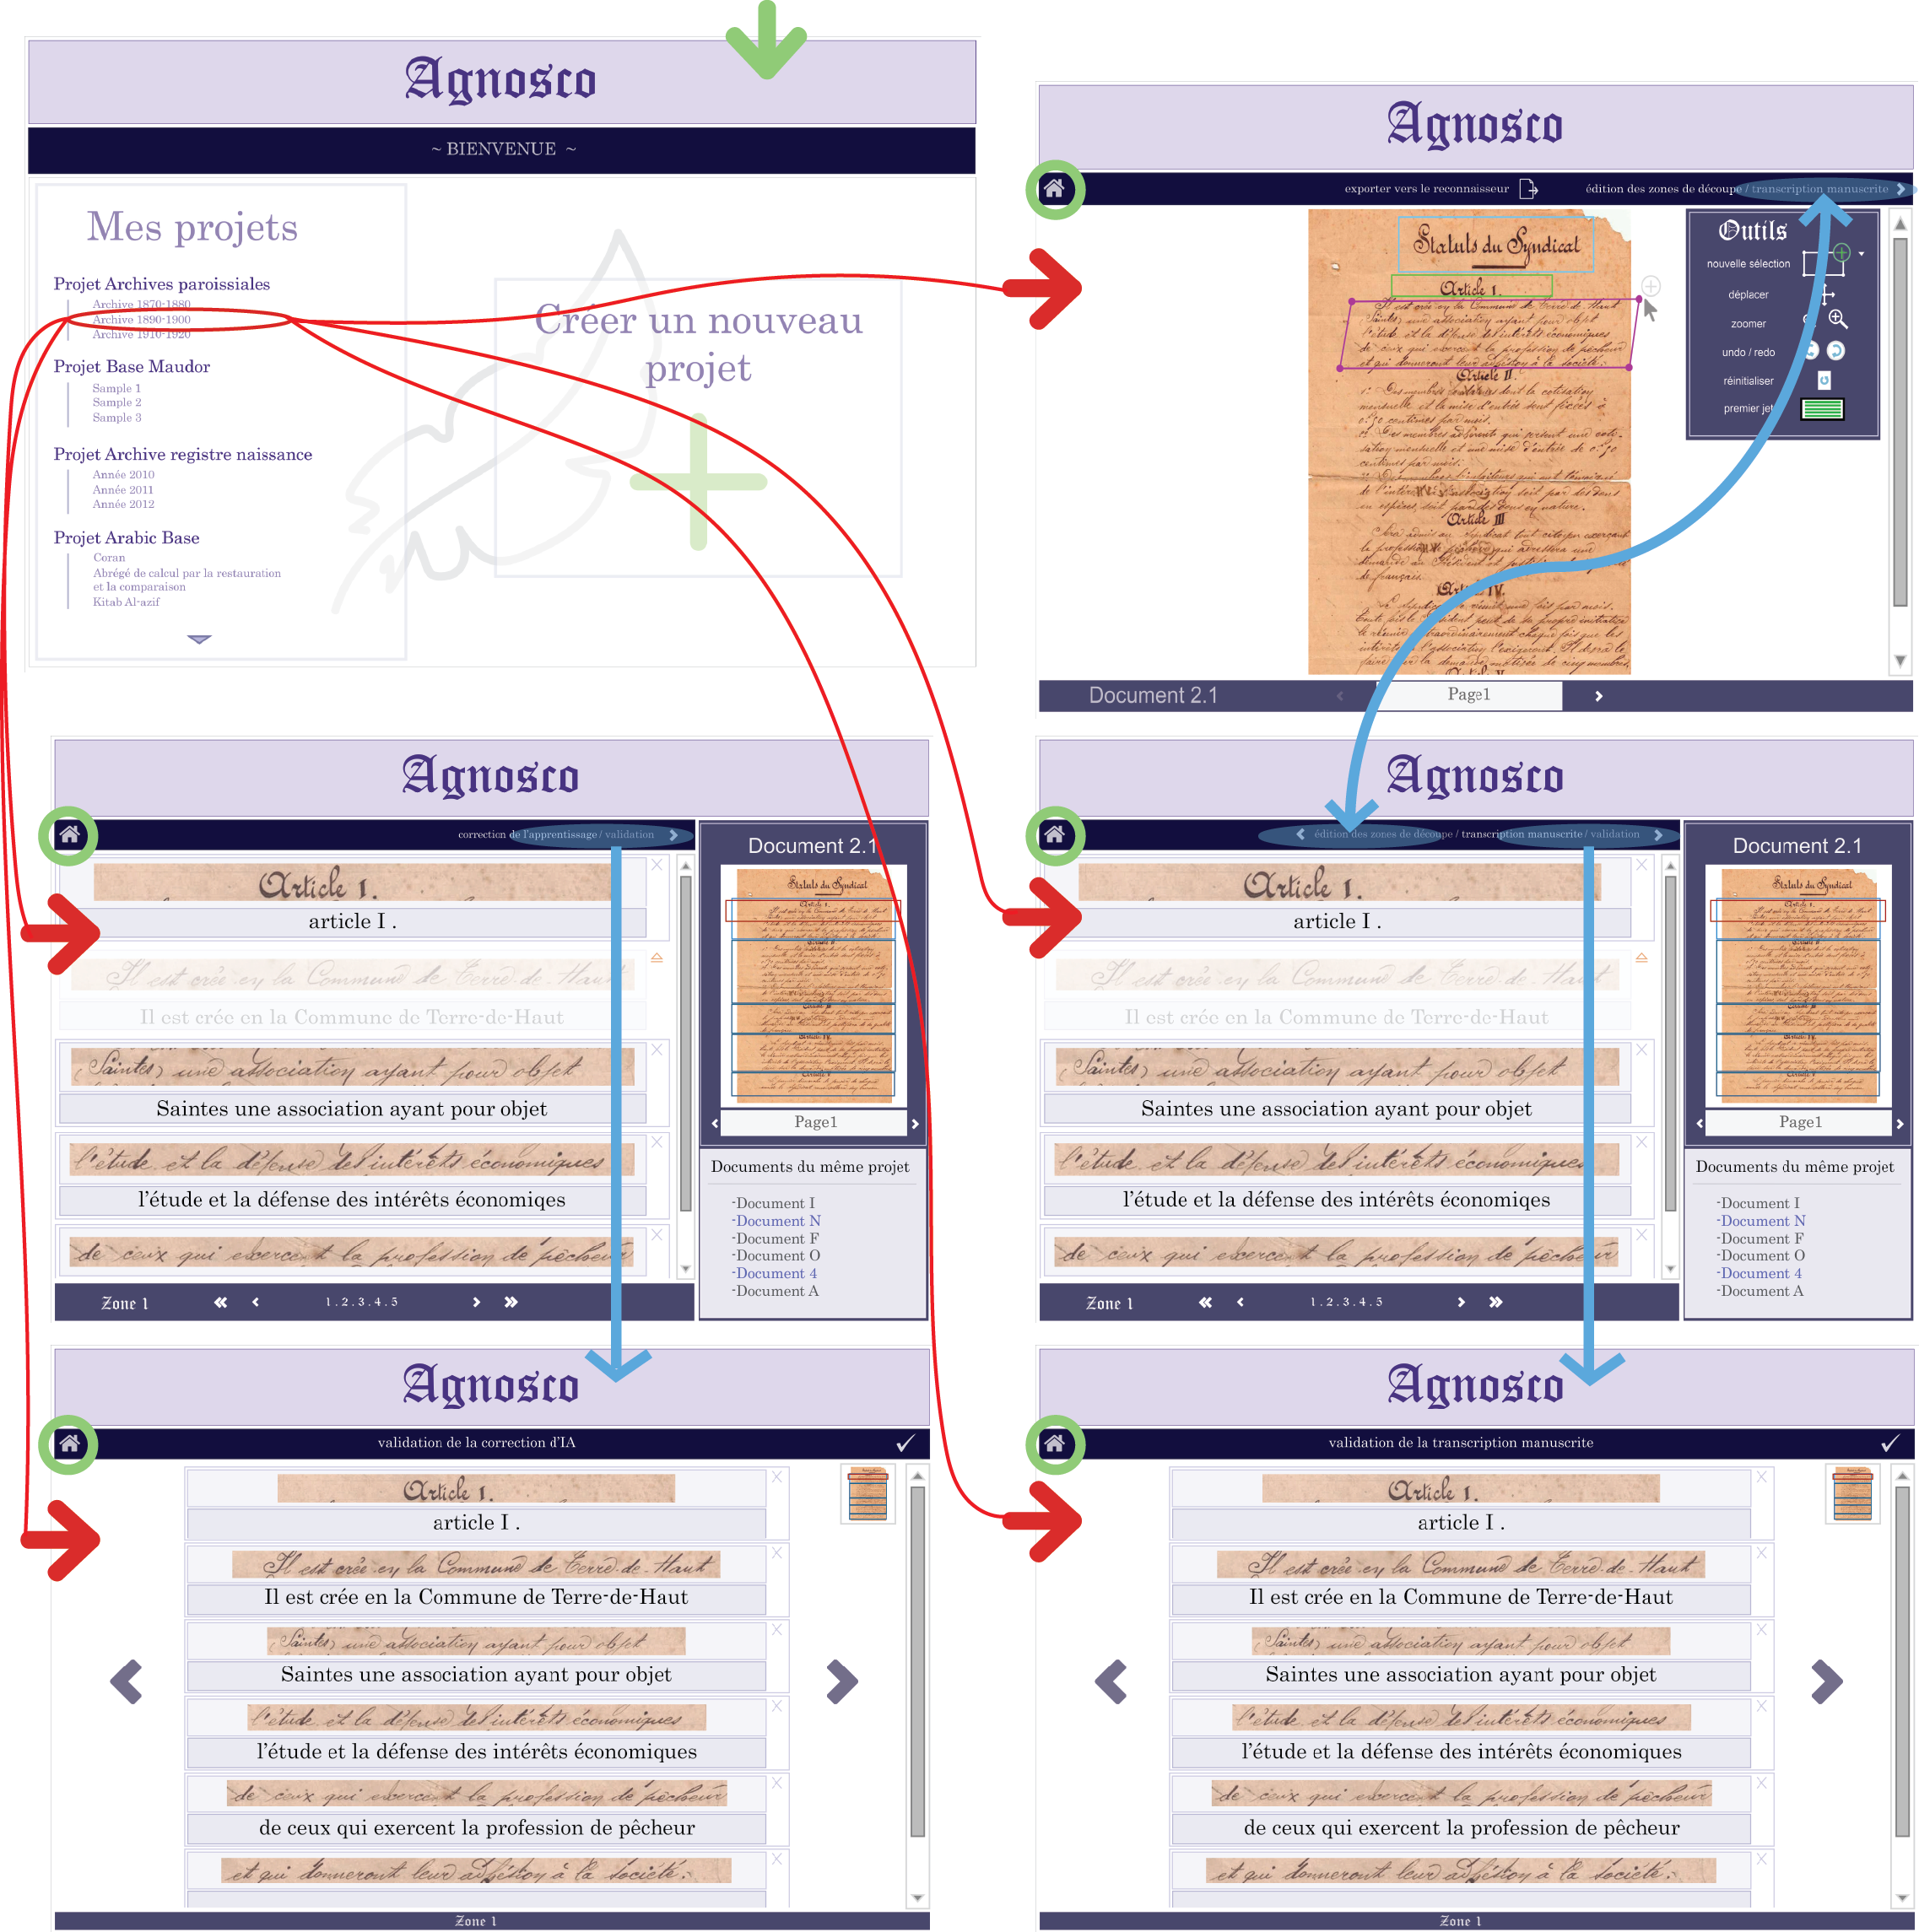
\includegraphics[scale=0.5]{assets/schemaIHMinteractions.png}
\end{center}
\end{mdframed}

\paragraph{Interactions entre le \textit{front-end} et le \textit{back-end}}

L’interface affiche les informations de la base de données (les couples imagettes - transcriptions) et les modifie. Pour ce faire, elle est reliée au connecteur central via sa ressource Rest. Le connecteur traite les demandes de l’IHM et les envoie au connecteur de la base de données. Celui-ci effectue les ordres de l’utilisateur sur la base et renvoie les imagettes et les transcriptions au connecteur central qui les fait suivre à l’IHM. Les modifications (ajout ou modification d’une transcription ou suppression d’un couple) sont enregistrées localement puis envoyées à la base de données lors du changement de page et du chargement d'une nouvelle page. Nous n'avons donc pas de bouton spécifique pour enregistrer les modifications.

\newpage{}

\paragraph{API Rest}
Pour communiquer avec le \textit{back-end}, nous utiliserons une API \texttt{Rest} dont les requêtes sont listées ci-dessous.
\newline{}

\begin{description}[align=left]

\item [Général]

\item [GET] \texttt{/base/projectsAndDocuments}\newline{}
\begin{itshape}
Renvoie la liste des noms des projets, contenant pour chaque projet une liste des noms des documents qui le composent.
\end{itshape}

\item [DELETE] \texttt{/base/deleteDocument/\{name\}}\newline{}
\begin{itshape}
Supprime le document de la base qui porte le nom donné, ainsi que son contenu.
\end{itshape}

\item [GET] \texttt{/base/availableRecognisers}\newline{}
\begin{itshape}
Renvoie la liste des noms des reconnaisseurs disponibles sur le serveur.
\end{itshape}

\item [POST] \texttt{/base/exportRecogniserExamples/\{name\}}\newline{}
\begin{itshape}
Récupère tous les exemples de la base qui sont contenus dans des projets utilisant le reconnaisseur dont le nom est passé en paramètre. Les exemples sont triés, ne sont retenus que ceux qui sont définis comme utilisables et validés. Ensuite, ces exemples sont exportés en tant que lot d'entraînement, vers le format d'entrée associé au reconnaisseur en question.
\end{itshape}

\item [Annotation / Validation]

\item [GET] \texttt{/base/documentPages/\{name\}}\newline{}
\begin{itshape}
Renvoie la liste des identifiants en base de données des pages qui composent un document dont le nom est donné en paramètre.
\end{itshape}

\item [GET] \texttt{/base/pageData/\{id\}}\newline{}
\begin{itshape}
Renvoie l'image associée à la page dont l'identifiant est donné en paramètre, ainsi que la liste des imagettes et des transcriptions des exemples qui la composent.
\end{itshape}

\item [POST] \texttt{/base/saveExampleEdits/}\newline{}
\begin{itshape}
Enregistre dans la base de données les modifications de transcriptions décrites par l'objet JSON associé à la requête.
\end{itshape}

\item [PUT] \texttt{/base/disableExample/\{id\}}\newline{}
\begin{itshape}
Rend l'exemple dont l'identifiant est donné en paramètre inutilisable, \textit{i.e.} l'utilisateur juge que l'image est trop parasitée ou que l'exemple n'est pas pertinent.
\end{itshape}

\item [PUT] \texttt{/base/enableExample/\{id\}}\newline{}
\begin{itshape}
Rend l'exemple dont l'identifiant est donné en paramètre utilisable (principalement utilisé pour annuler l'action décrite ci-dessus).
\end{itshape}

\item [POST] \texttt{/base/validateExamples/}\newline{}
\begin{itshape}
Valide tous les exemples dont les identifiants sont fournis dans une liste JSON associée à la requête.
\end{itshape}

\item [Découpe]

\item [GET] \texttt{/base/documentPagesWithImages/\{name\}}\newline{}
\begin{itshape}
Renvoie la liste des identifiants et des images associés aux pages qui composent le document portant le nom donné.
\end{itshape}

\item [POST] \texttt{/base/addDocumentGroundtruth/\{name\}}\newline{}
\begin{itshape}
Ajoute à la base la vérité terrain donnée dans l'objet PiFF (donc JSON) associé à la requête, et l'associe au document dont le nom est donné en paramètre.
\end{itshape}

\item [GET] \texttt{/base/recogniseImages/\{name\}}\newline{}
\begin{itshape}
Envoie la liste des imagettes contenues dans le document donné au reconnaisseur associé au projet contenant ce document. La réponse à cette requête est une liste de transcriptions trouvées par le reconnaisseur.
\end{itshape}

\end{description}